\subsection{Procedurální generace počítačového rozhraní}
\label{sec:generace_rozhrani}

Po výše zmíněné generaci mapy je třeba umístit na mapu jednotlivé počítače. Je tak učiněno opět za pomocí několika možných pozic umístění. Každý počítač je identifikován fiktivním jménem jeho vlastníka. Toto jméno je generováno z předvytvořeného pole. Po umístění PC na mapu je generováno počítačové rozhraní.

Počítačové rozhraní je pro každý počítač na mapě generováno unikátně. Rozhraní je inspirováno Linuxovým rozhraním.

Na levé straně simulovaného počítačového rozhraní se nacházejí soubory, jejichž jména, ikony a koncovky jsou náhodně generovány.

Původně byly soubory náhodně rozmístěny po celé ploše. Tento přístup byl však matoucí a ani příliš neodpovídal situacím z reálného světa. Je sice pravdou, že systémy jako je MacOS umožňují umísťovat soubory libovolně po celé ploše, většinou však uživatelé stejně dodržují určitou systematičnost v jejich rozmístění. Proto bylo rozhodnuto, že soubory budou rozmístěny do sloupců na levé části obrazovky.

Prvním krokem generace je výběr aktuálního sloupce. Na začátku se tedy jedná o~sloupec s indexem nula. Následně je vybrán náhodný počet souborů, které budou v sloupci vytvořeny.

V dalším kroku je vybrána textura souboru z již existujících textur. Odpovídající textuře je přiřazen název z existujícího pole názvů a odpovídající přípona. Jedním z~prvků je taktéž možnost, že je soubor škodlivý. To lze poznat podle podezřelého názvu nebo přípony. V takovém případě je úkolem uživatele soubor smazat.

Tento proces je opakován v každém ze sloupců.

\begin{figure}[ht]
    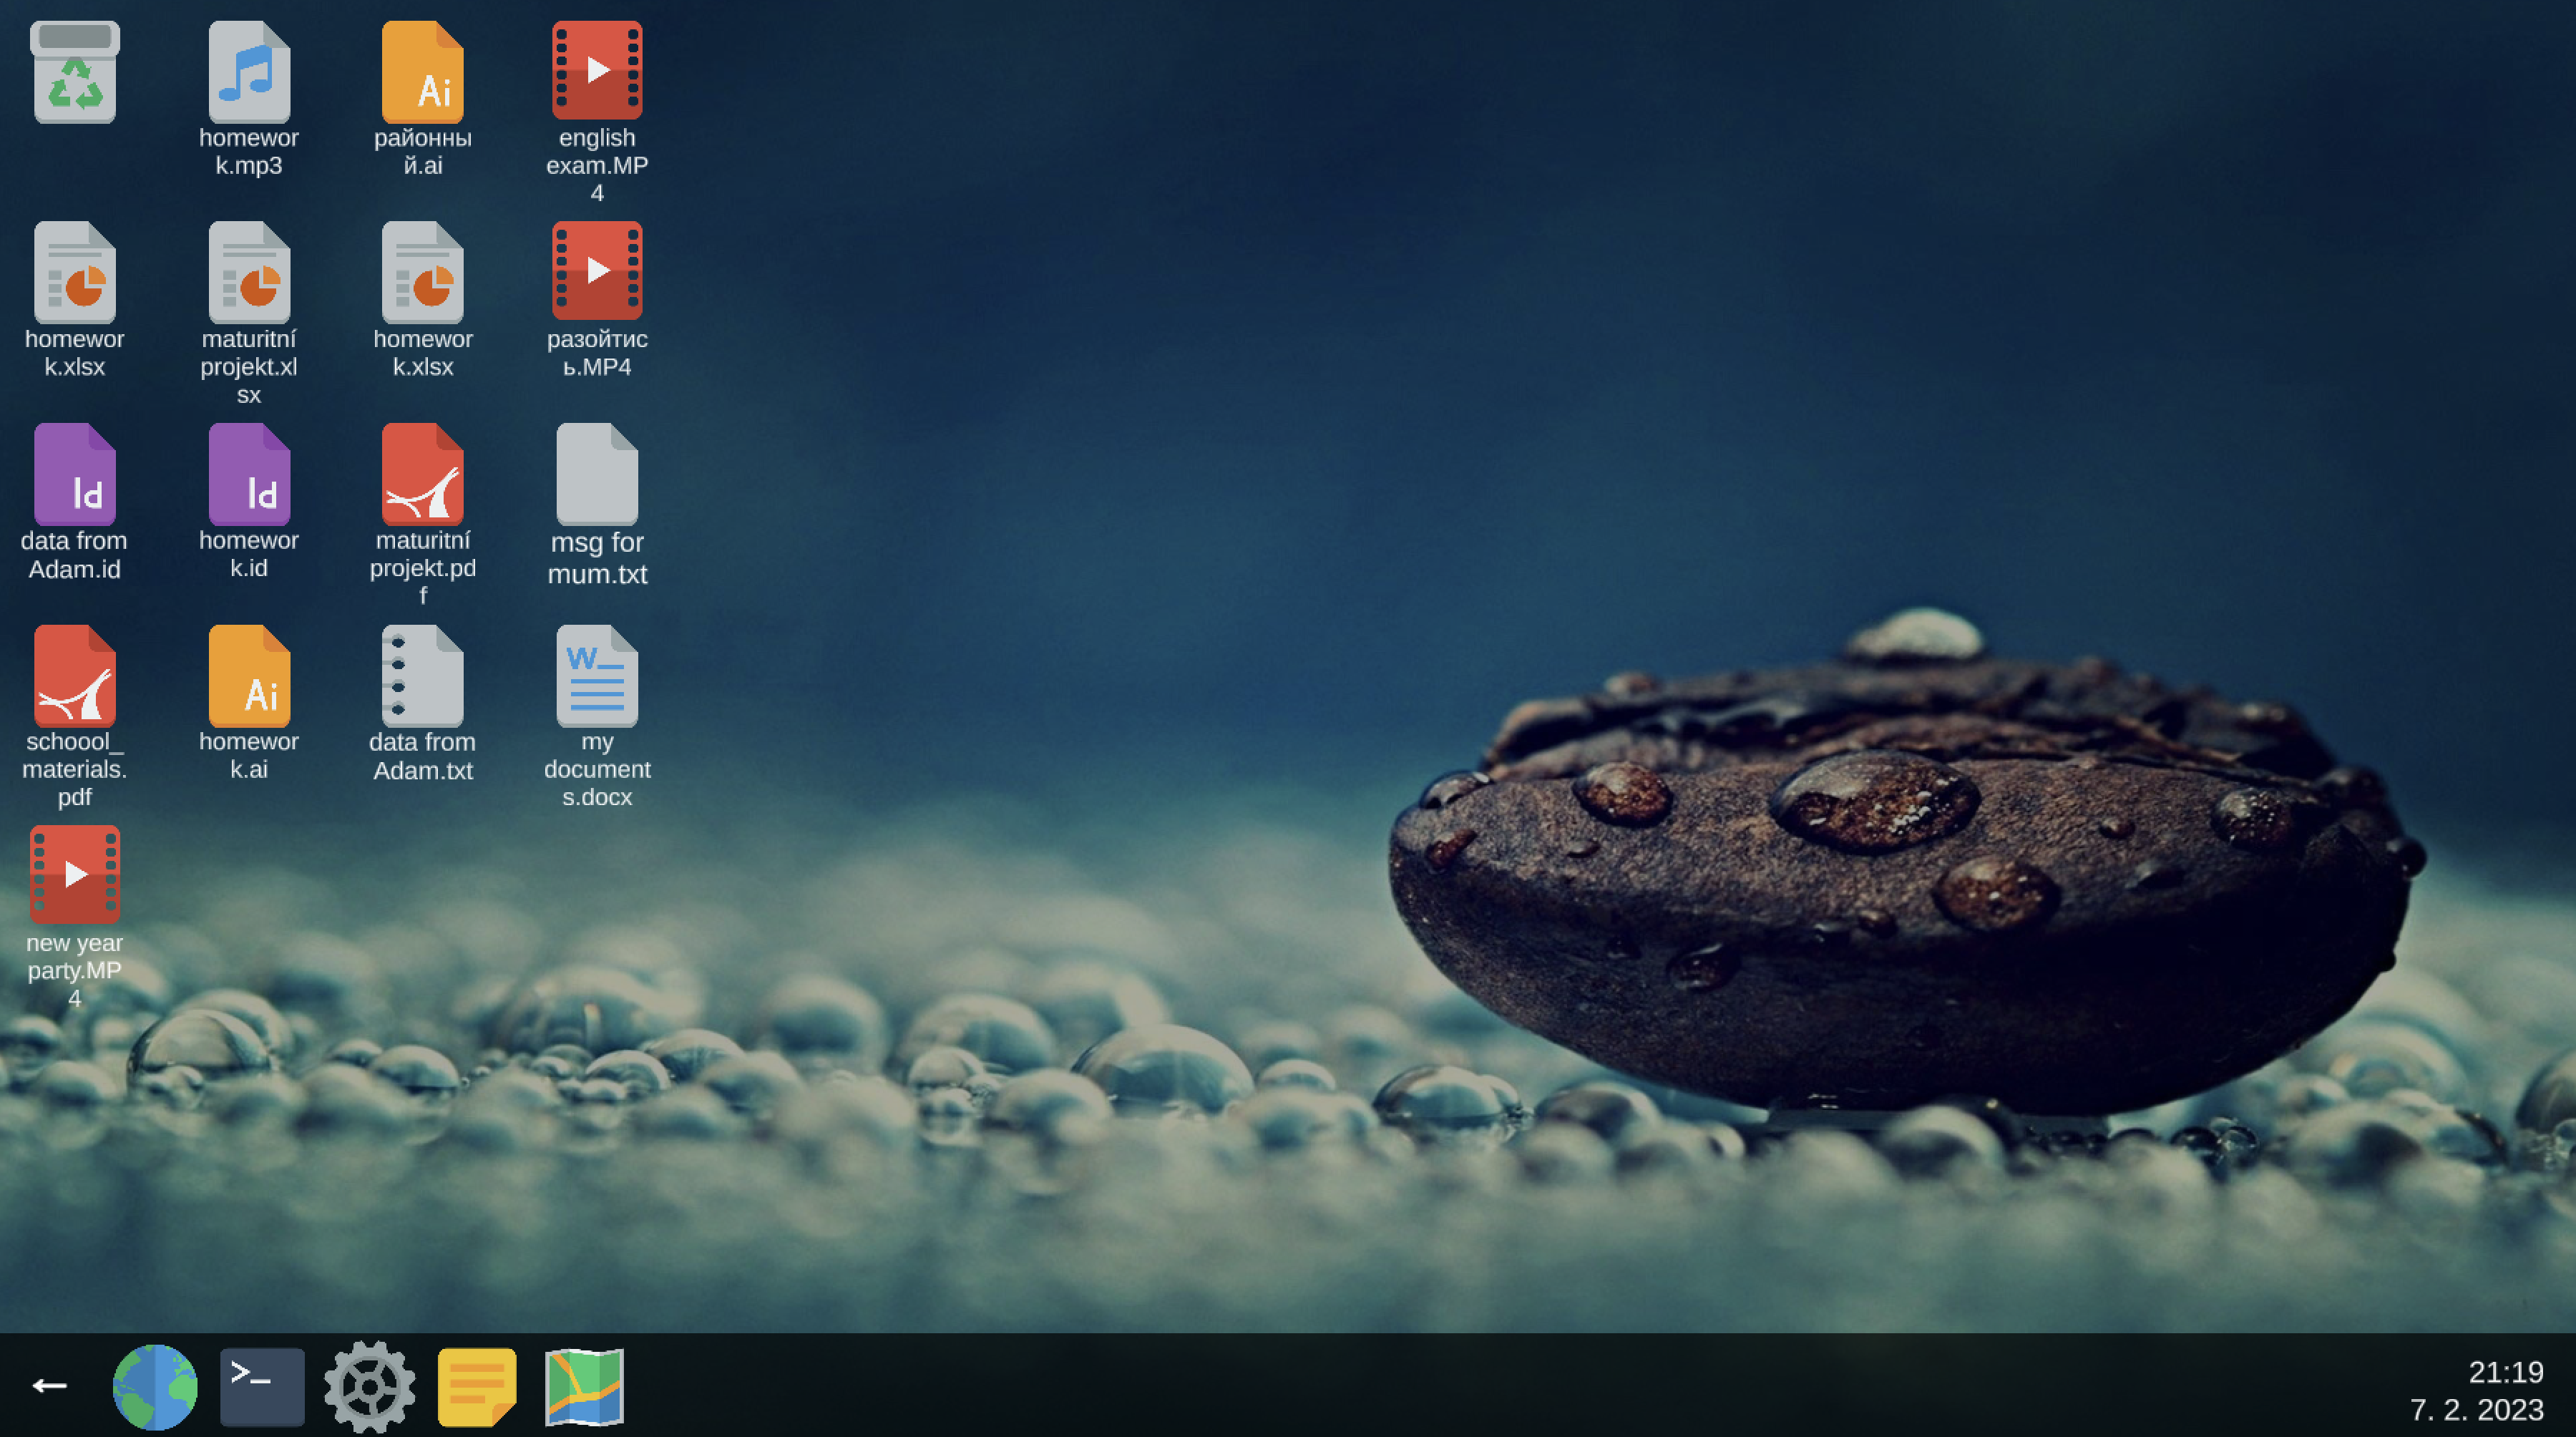
\includegraphics[width=\columnwidth]{pc0.png}
    \centering
    \caption{Ukázka grafického vzhledu počítačového rozhraní}
    \label{fig:pc0_img}
\end{figure}

\begin{figure}[ht]
    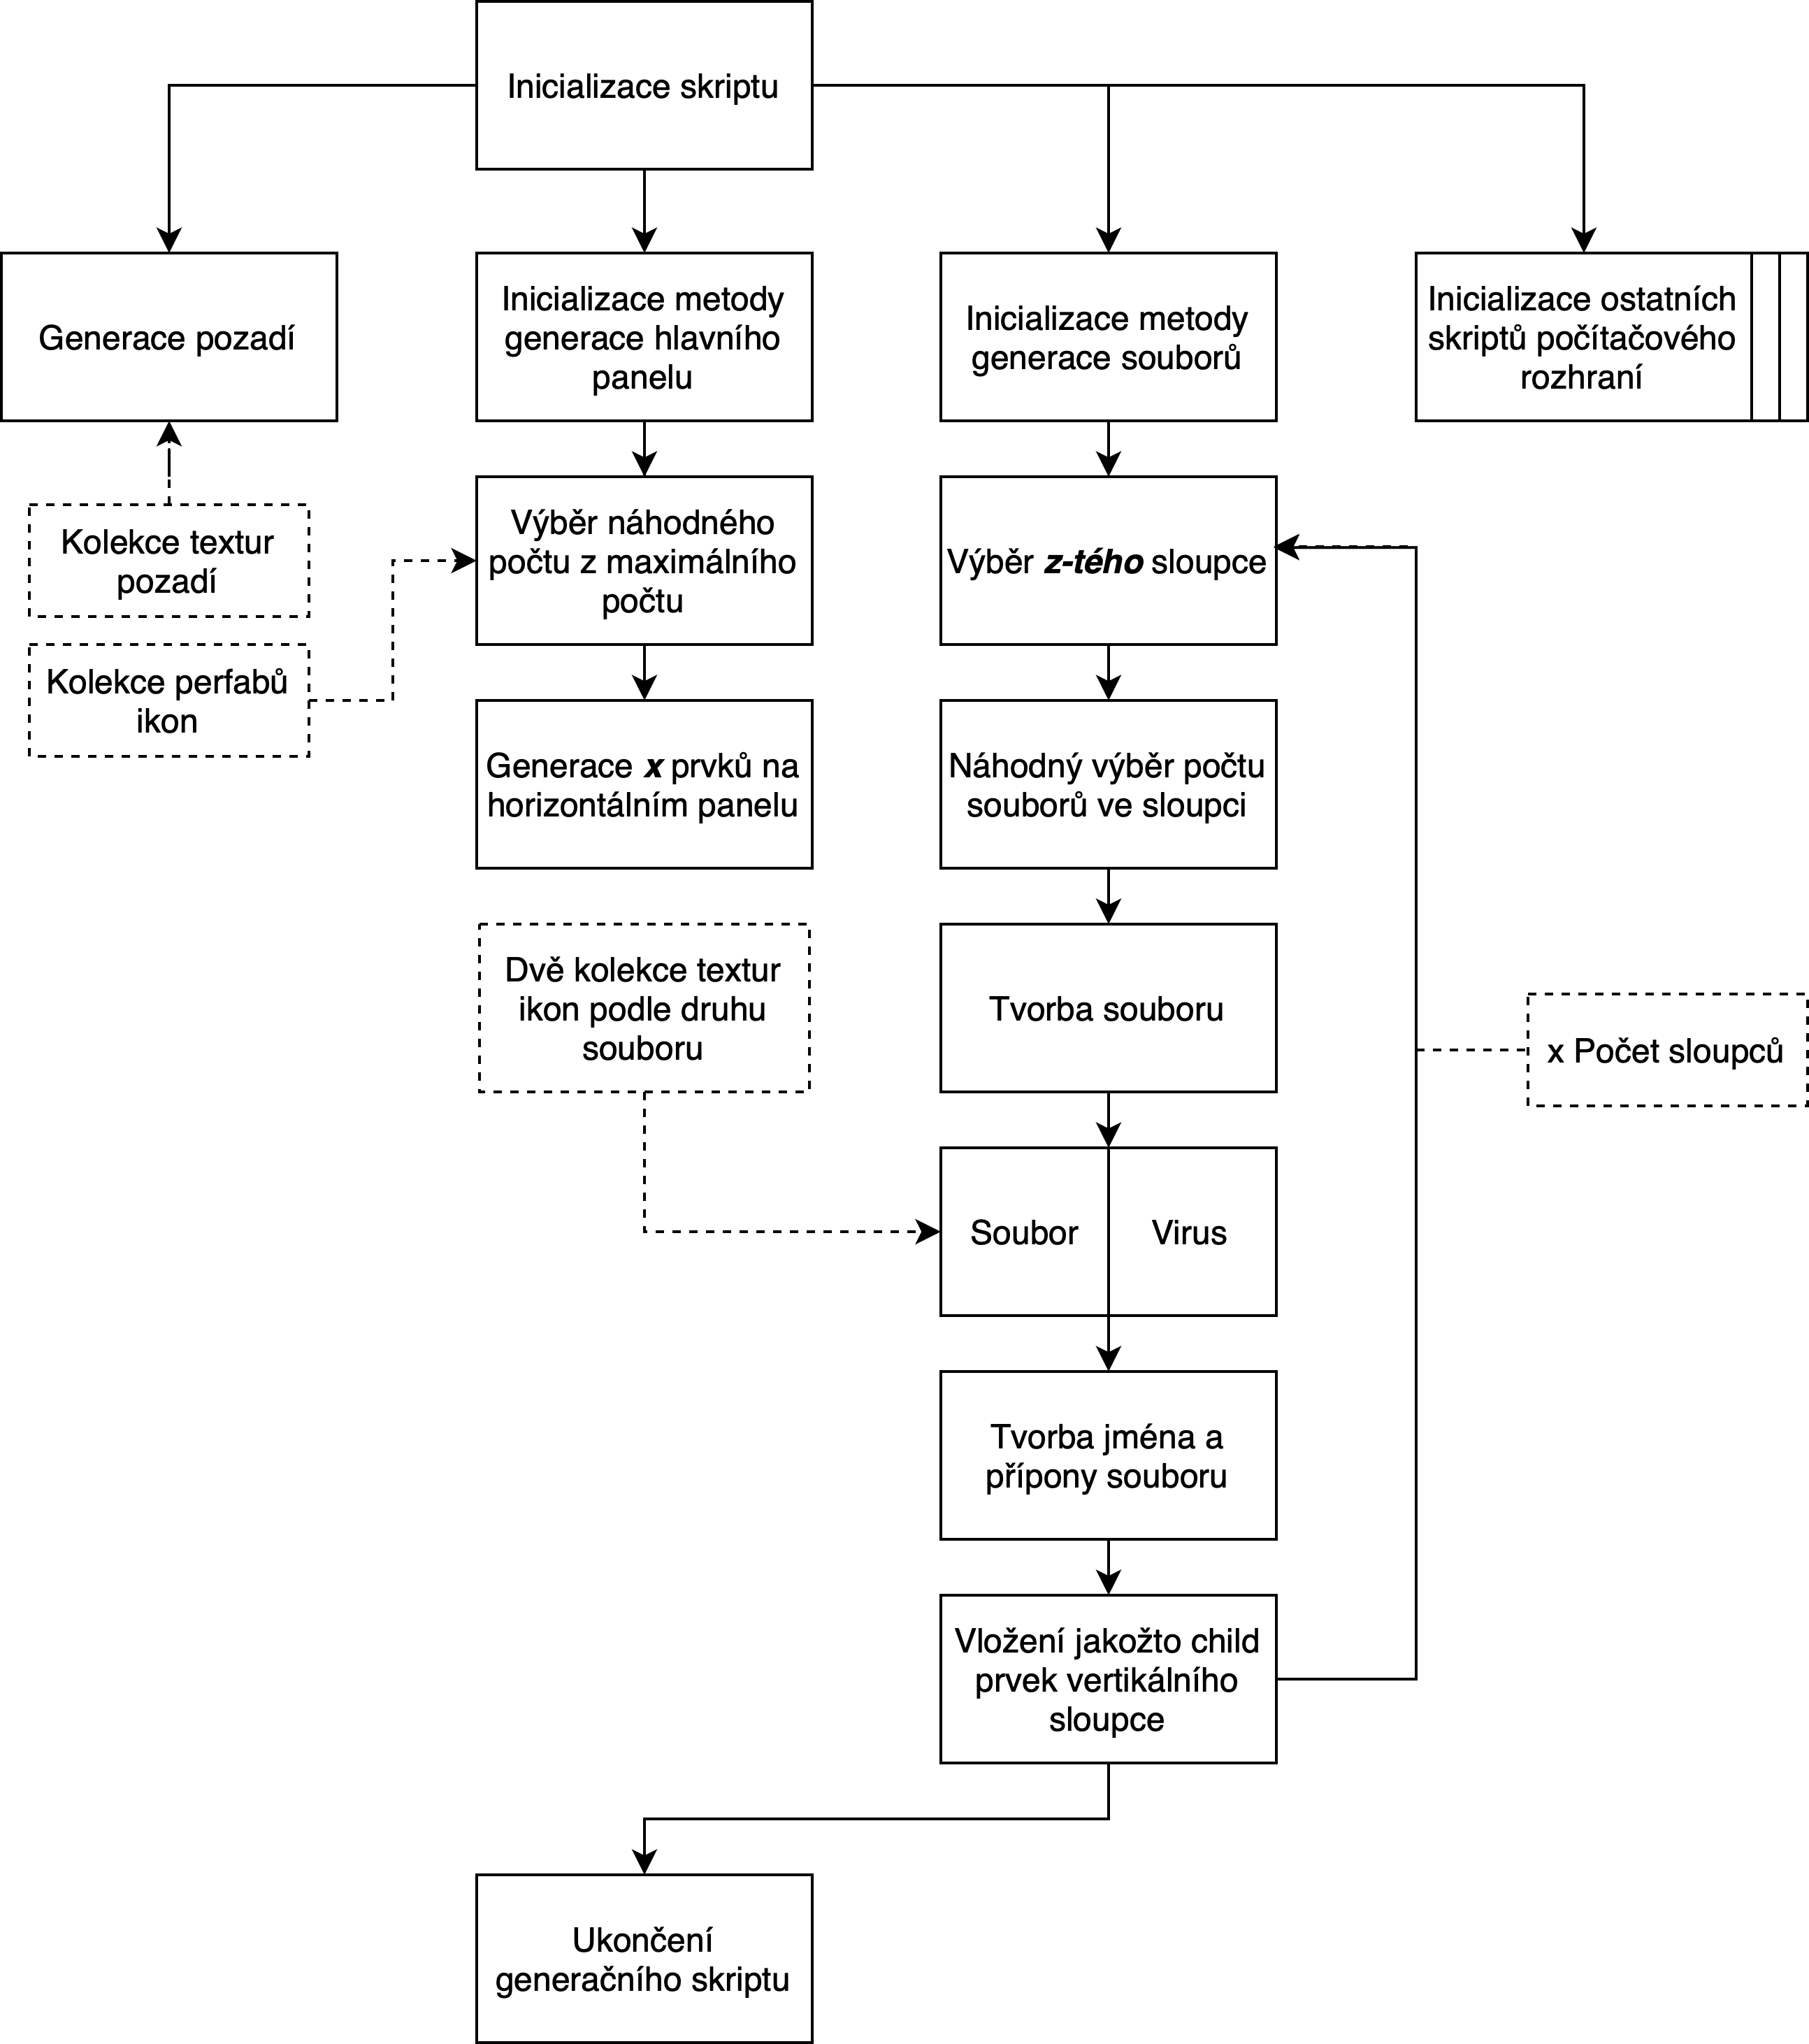
\includegraphics[width=\columnwidth]{generace_ui.png}
    \centering
    \caption{Znázornění generování grafického rozhraní}
    \label{fig:generace_ui_img}
\end{figure}
